\documentclass{beamer}

\usepackage{graphicx}
%\usepackage{beamerthemesplit}
\usetheme{Boadilla}
\usecolortheme{seahorse}%crane}
%\usefonttheme[onlymath]{serif}

\title[Transfer functions]{Transfer functions --- Weighted averaging and all that}
\author[Gavin Simpson]{Gavin Simpson \\ (\texttt{gavin.simpson@ucl.ac.uk})}
\institute[Aarhus]{Aarhus University}
\date[ACME 2008]{ACME 2022}

\usepackage{Sweave}
\begin{document}

\begin{frame}
\titlepage
\end{frame}

\section*{Outline}
\begin{frame}
 \frametitle{Outline}
 \tableofcontents
\end{frame}

\section{Motivating Examples}
\begin{frame}
    \frametitle{Example 1: Was acid rain to blame for acid lakes?}
    \begin{itemize}
        \item In the 1970s and early 1980s there was a great deal of concern about acid lakes and rivers in northern Europe
        \item Driven mainly by losses of Salmon in Scandinavian rivers, this was a major political hot potato
        \item A vast amount of money was expended to determine the cause of the acidification --- was it due to acid emissions from power stations or some other cause?
        \item Palaeolimnological data provided conclusive proof that acid deposition was the cause
        \item In Europe, the Surface Waters Acidification Project (SWAP) was a major contributor to the debate
        \item Diatoms collected from 167 lakes across UK, Norway, Sweden and associated water chemistry
        \item Can we predict lake-water pH from the diatom species assemblages?
        \item Apply to diatoms counted from a sediment core from the Round Loch of Glenhead (RLGH) covering most of the Holocene
    \end{itemize}
\end{frame}

\begin{frame}
    \frametitle{Example 2: Reconstructing past sea surface temperatures}
    \begin{itemize}
        \item Sea surface temperatures are related to global air temperatures
        \item An important arm of palaeoceanography is involved in reconstructing past climates from various proxies
        \item These past climates tell use how the world responded to previous climatic shifts and provide targets for climate modellers to try to model
        \item The data set here is the Imbrie \& Kipp data set --- the data set that started it all!
        \item 61 core-top samples from ocean cores, mainly from Atlantic
        \item 27 species of planktonic foraminifera were identified in the core-top samples
        \item Summer and Winter sea surface temperatures (SST) and sea water salinity values measured at each of the 61 core locations
        \item Applied to reconstruct SST and salinity for 110 samples from Core V12-133 from the Caribbean
    \end{itemize}
\end{frame}

% \begin{frame}
%     \frametitle{Example 3: Modern reference sites for UK acid lakes}
%     \begin{itemize}
%         \item 
%     \end{itemize}
% \end{frame}

\section{Introduction}
\begin{frame}
    \frametitle{Palaeoecological transfer functions}
    \begin{columns}
    
    \column{7cm}
    \begin{itemize}
        \item Transfer functions
        \item Calibration
        \item Bioindication
        \item Aim is to predict the environment from observations on species environment
        \item The reverse of constrained ordination from yesterday
        \item ter Braak (1995) \emph{Chemometrics and Intelligent Laboratory Systems} \textbf{28}: 165--180
    \end{itemize}
    
    \column{5cm}
    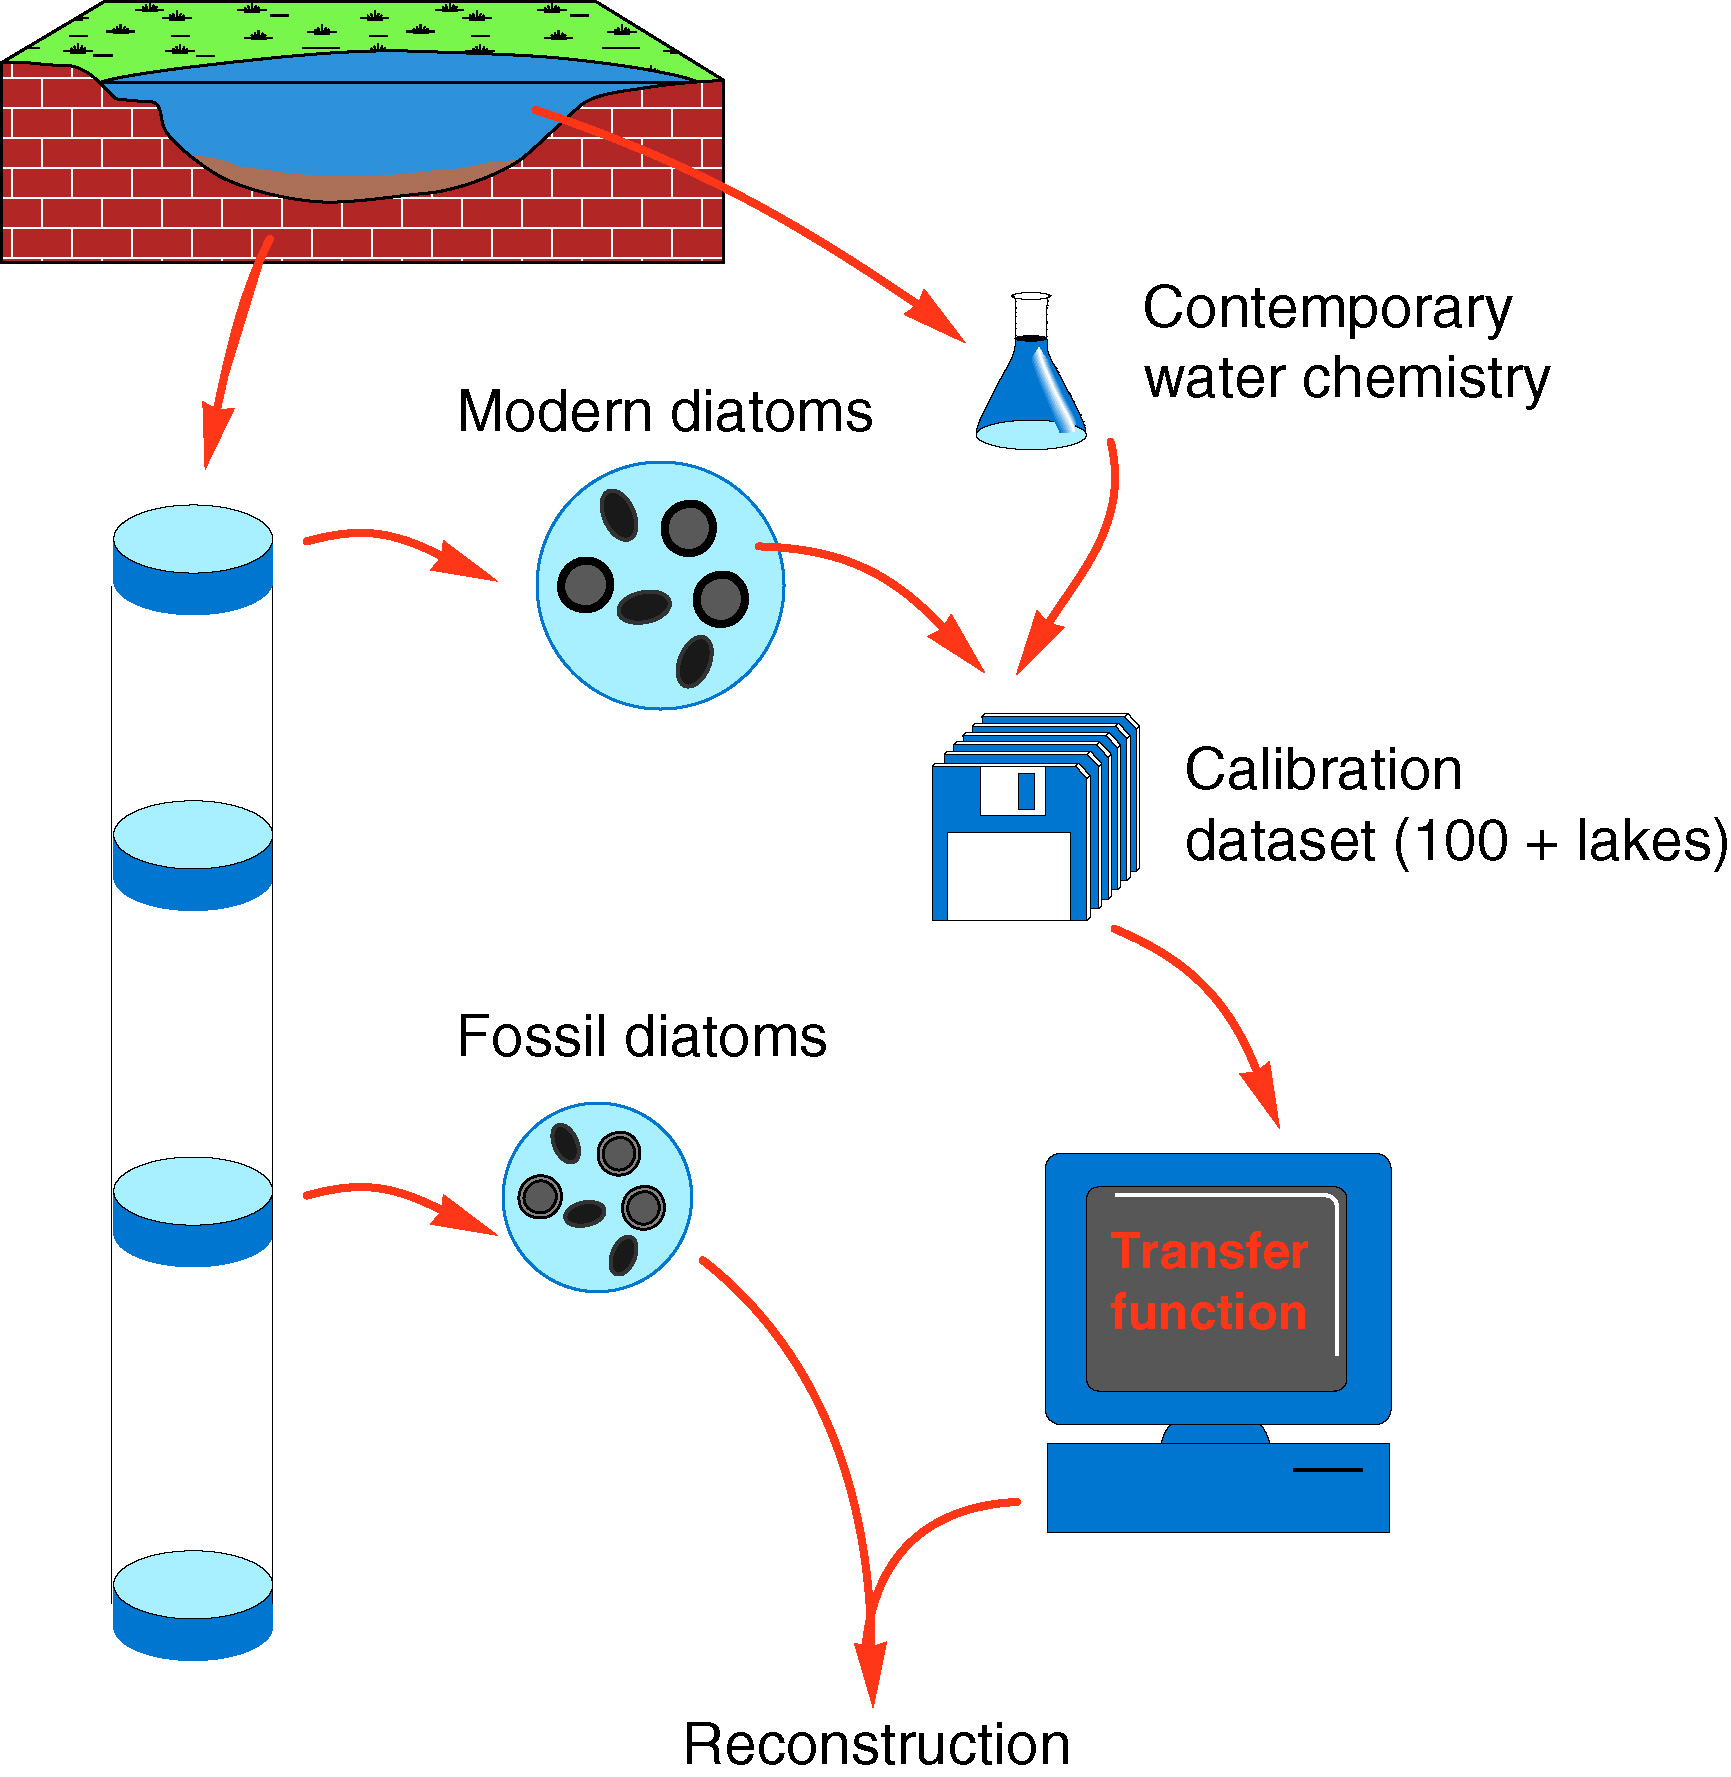
\includegraphics[width=5cm]{transferfunction}
    \end{columns}
\end{frame}

\begin{frame}
    \frametitle{Palaeoecological transfer functions}
    \begin{itemize}
        \item More formally we have
        \begin{itemize}
            \item Matrix of species abundances, $\mathbf{Y}$
            \item Vector of observations of an environmental variable, $\mathbf{x}$
        \end{itemize}
        \item Assume $\mathbf{Y}$ is some function $f$ of the environment plus an error term
        $$\mathbf{Y} = f(\mathbf{x}) + \varepsilon$$
        \item In the \alert{classical} approach $f$ is estimated via regression of $\mathbf{Y}$ on $\mathbf{x}$
        \item Then invert $f$, ($f^{-1}$) to yield estimate of environment $\mathbf{x_0}$ from fossil species assemblage $\mathbf{y_0}$
        $$\mathbf{\hat{x}_0} = f(\mathbf{y_0})^{-1}$$
        \item In all but simplest cases $f^{-1}$ doesn't exist and must be estimated via optimisation
    \end{itemize}

\end{frame}

\begin{frame}
    \frametitle{Palaeoecological transfer functions}
    \begin{itemize}
        \item To avoid problems of inverting $f$, the \alert{indirect} approach directly estimates the inverse of $f$, here $g$, from the data by regression $\mathbf{x}$ on $\mathbf{Y}$
        $$\mathbf{x} = g(\mathbf{Y}) + \varepsilon$$
        \item We do \alert{not} believe that the species influence their environment!
        \item This is just a trick to avoid having to estimate $f$
        \item The predicted environment for a fossil sample $\mathbf{y_0}$ is
        $$\mathbf{\hat{x}_0} = g(\mathbf{y_0})$$
    \end{itemize}
\end{frame}

\begin{frame}
    \frametitle{Assumptions of palaeoecological transfer functions}
    \begin{itemize}
        \item Taxa in training set are systematically related to the environment in which they live
        \item Environmental variable to be reconstructed is, or is linearly related to, an ecologically important variable in the ecosystem
        \item Taxa in the training set are the same as in the fossil data and their ecological responses have not changed significantly over the timespan represented by the fossil assemblages
        \item Mathematical methods used in regression and calibration adequately model the biological responses to the environment
        \item Other environmental variables have negligible influence, or their joint distribution with the environmental variable of interest is the same as in the training set
        \item In model evaluation by cross-validation, the test data are independent of the training data --- the \alert{secret assumption} until Telford \& Birks (2005)
    \end{itemize}
\end{frame}

\begin{frame}
    \frametitle{Different types of transfer functions}
    \begin{itemize}
        \item There are a large number of transfer function models
        \item Many motivated from chemometrics, but modified to deal with non-linear species responses
        \item Partial least squares (PLS) and WA-PLS
        \item Mutual Climate Range method
        \item So-called maximum likelihood method (Multivariate Gaussian logistic regression)
        \item Two of the most used (except WA-PLS) are
        \begin{itemize}
            \item Weighted Averaging (WA)
            \item Modern Analogue Technique (MAT)
            \item These are the two techniques we will investigate today
        \end{itemize}
        \item Large number of potential techniques from machine learning, bioinformatics, that have yet to be investigated
    \end{itemize}
\end{frame}

\section{Weighted Averaging}
\begin{frame}
    \frametitle{Weighted averaging}
    \begin{itemize}
        \item Species don't respond in simple ways to \emph{environmental gradients}
        \item Maximum likelihood method fitted Gaussian curves to each species and then numerical optimisation used to predict for fossil samples
        \item Computationally very intensive, especially when doing cross-validation
        \item Weighted averaging is an approximation to this maximum likelihood approach
    \end{itemize}
    \begin{center}
        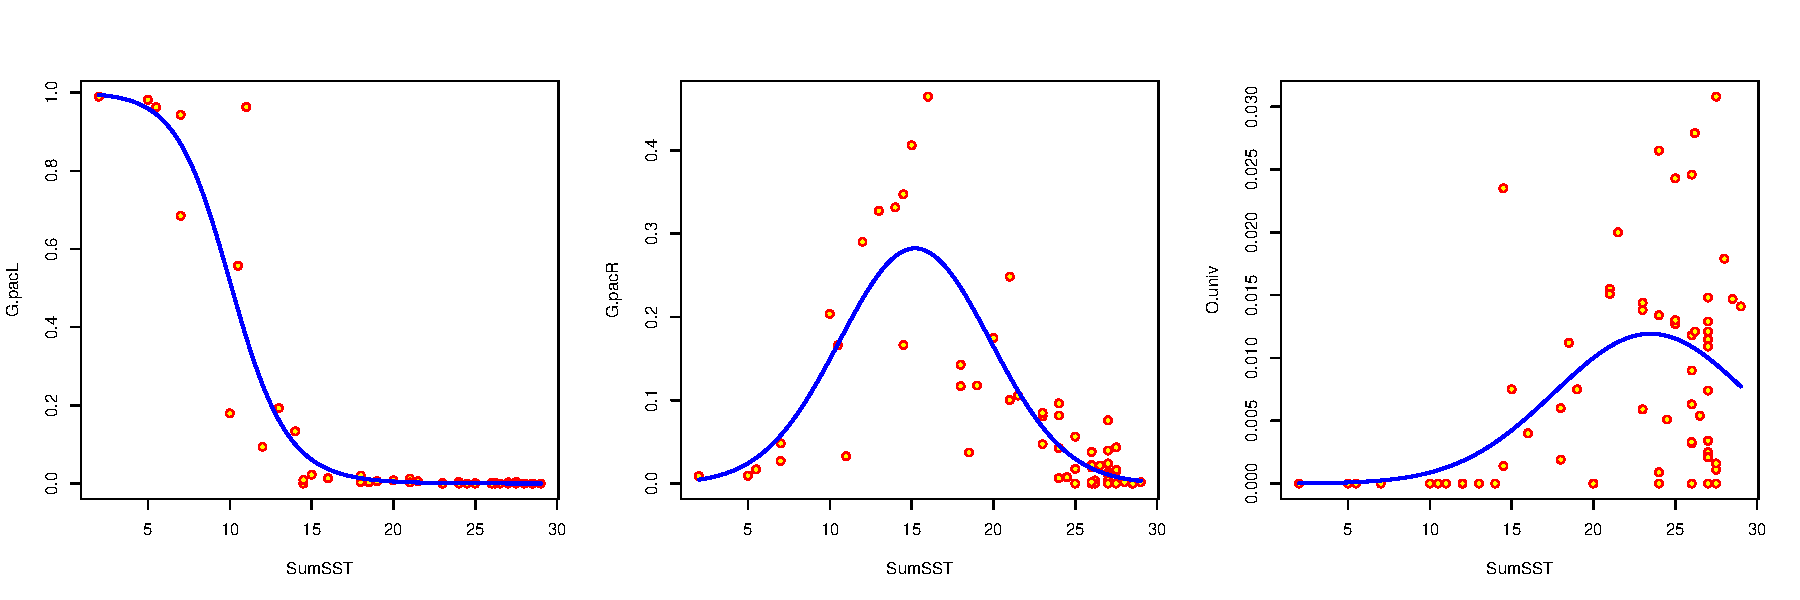
\includegraphics[width=10cm]{three_forams_gauss}
    \end{center}
\end{frame}

\begin{frame}
    \frametitle{Weighted averaging}
    \begin{columns}
    \column{7cm}
    \begin{itemize}
        \item A very simple idea
        \item In a lake, with a certain pH, a species with their pH optima close to the pH of the lake will tend to be the most abundant species present
        \item A simple estimate of the a species' pH optimum is an average of all the pH values for lakes in which that species occurs, weighted by their abundance
        \item An estimate of a lake's pH is the weighted average of the pH optima of all the species present, again weighted by species abundance
    \end{itemize}
    
    \column{5cm}
    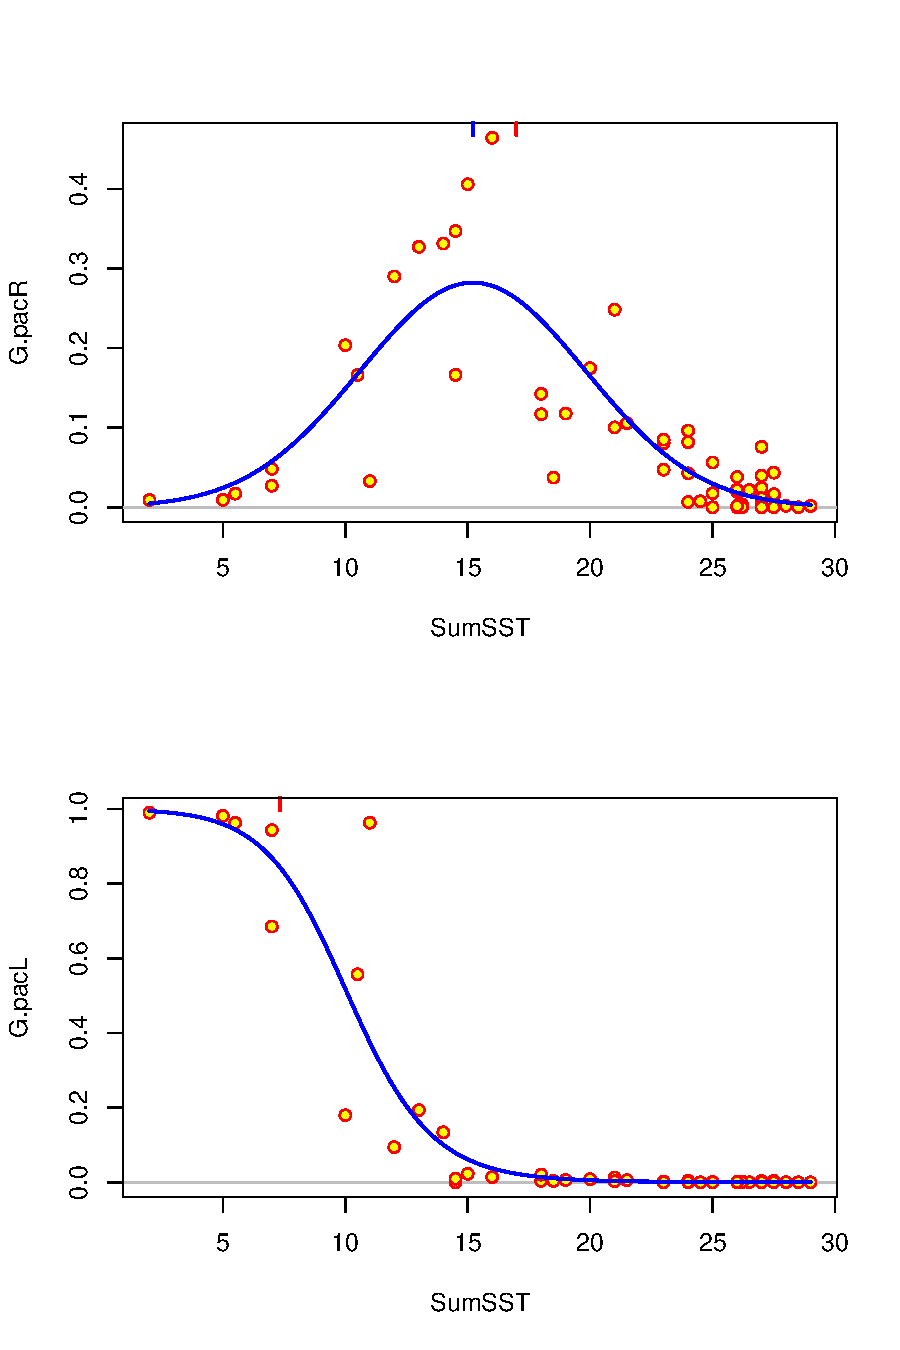
\includegraphics[width=5cm]{g_pachy_wa}
    \end{columns}
\end{frame}

\begin{frame}
    \frametitle{Deshrinking}
    \begin{columns}
        \column{7.5cm}
        \begin{itemize}
            \item By taking averages twice, the range of predicted values is smaller than the observed range
            \item Deshrinking regressions stretch the weighted averages back out to the observed range
            \item Can do \alert{inverse} or \alert{classical} regressions
            \begin{itemize}
                \item inverse: regress gradient values on WA's
                \item classical: regress WA's on gradient values
                \item Vegan also allows to just make variances equal
            \end{itemize}
            \item Inverse and classical regression remove both bias and error, equalising variances deshrinks without adjusting the bias
        \end{itemize}

        \column{5cm}
        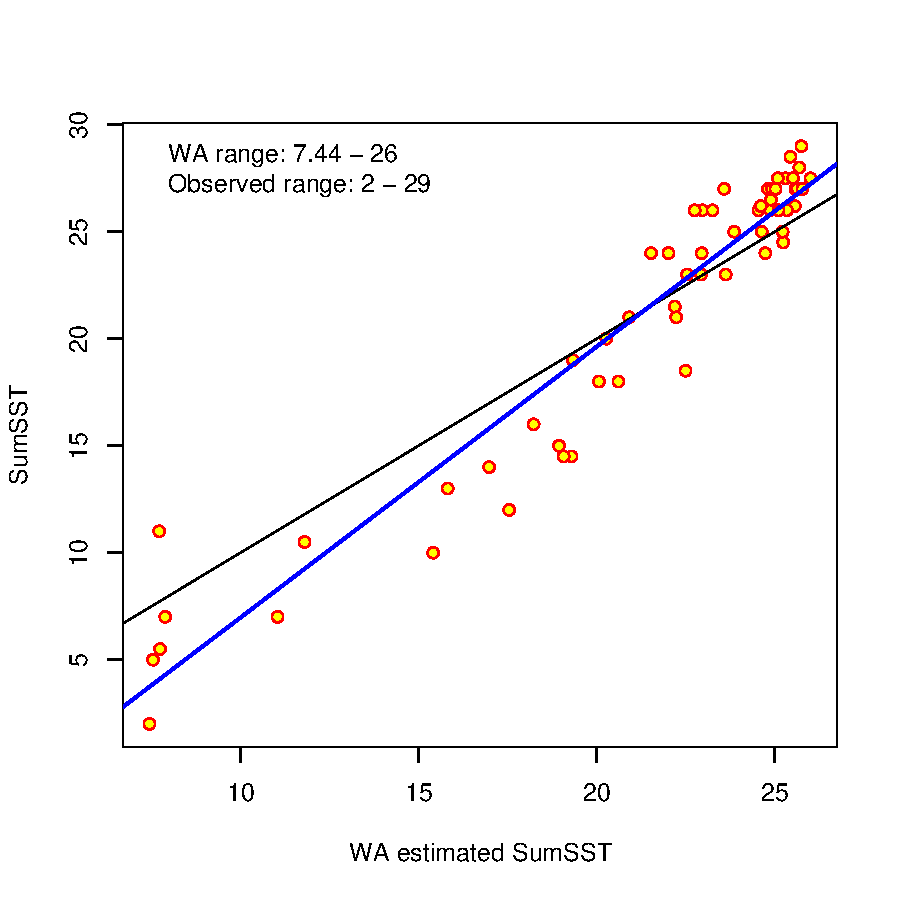
\includegraphics[width=5cm]{deshrinking}
    \end{columns}
\end{frame}

\begin{frame}[fragile]
    \frametitle{WA in analogue}
    \begin{itemize}
        \item \textbf{analogue} contains \textsf{R} code for fitting WA transfer functions and associated helper functions
    \end{itemize}
    \scriptsize
\begin{Schunk}
\begin{Sinput}
r$> SumSST <- imbrie.env$SumSST
r$> mod <- wa(SumSST ~ ., data = imbrie, deshrink = "inverse")
r$> mod
\end{Sinput}
\begin{Soutput}
	Weighted Averaging Transfer Function

Call:
wa(formula = SumSST ~ ., data = imbrie, deshrink = "inverse") 

Deshrinking  : Inverse 
Tolerance DW : No 
No. samples  : 61 
No. species  : 27 

Performance:
     RMSE  R-squared  Avg. Bias  Max. Bias  
   2.0188     0.9173     0.0000    -3.8155  
\end{Soutput}
\end{Schunk}
    \normalsize
\end{frame}

\begin{frame}[fragile]
    \frametitle{WA --- diagnostic plots}
    \scriptsize
\begin{Schunk}
\begin{Sinput}
r$> opar <- par(mfrow = c(1,2))
r$> plot(mod)
r$> par(opar)
\end{Sinput}
\end{Schunk}
    \normalsize
    \begin{center}
    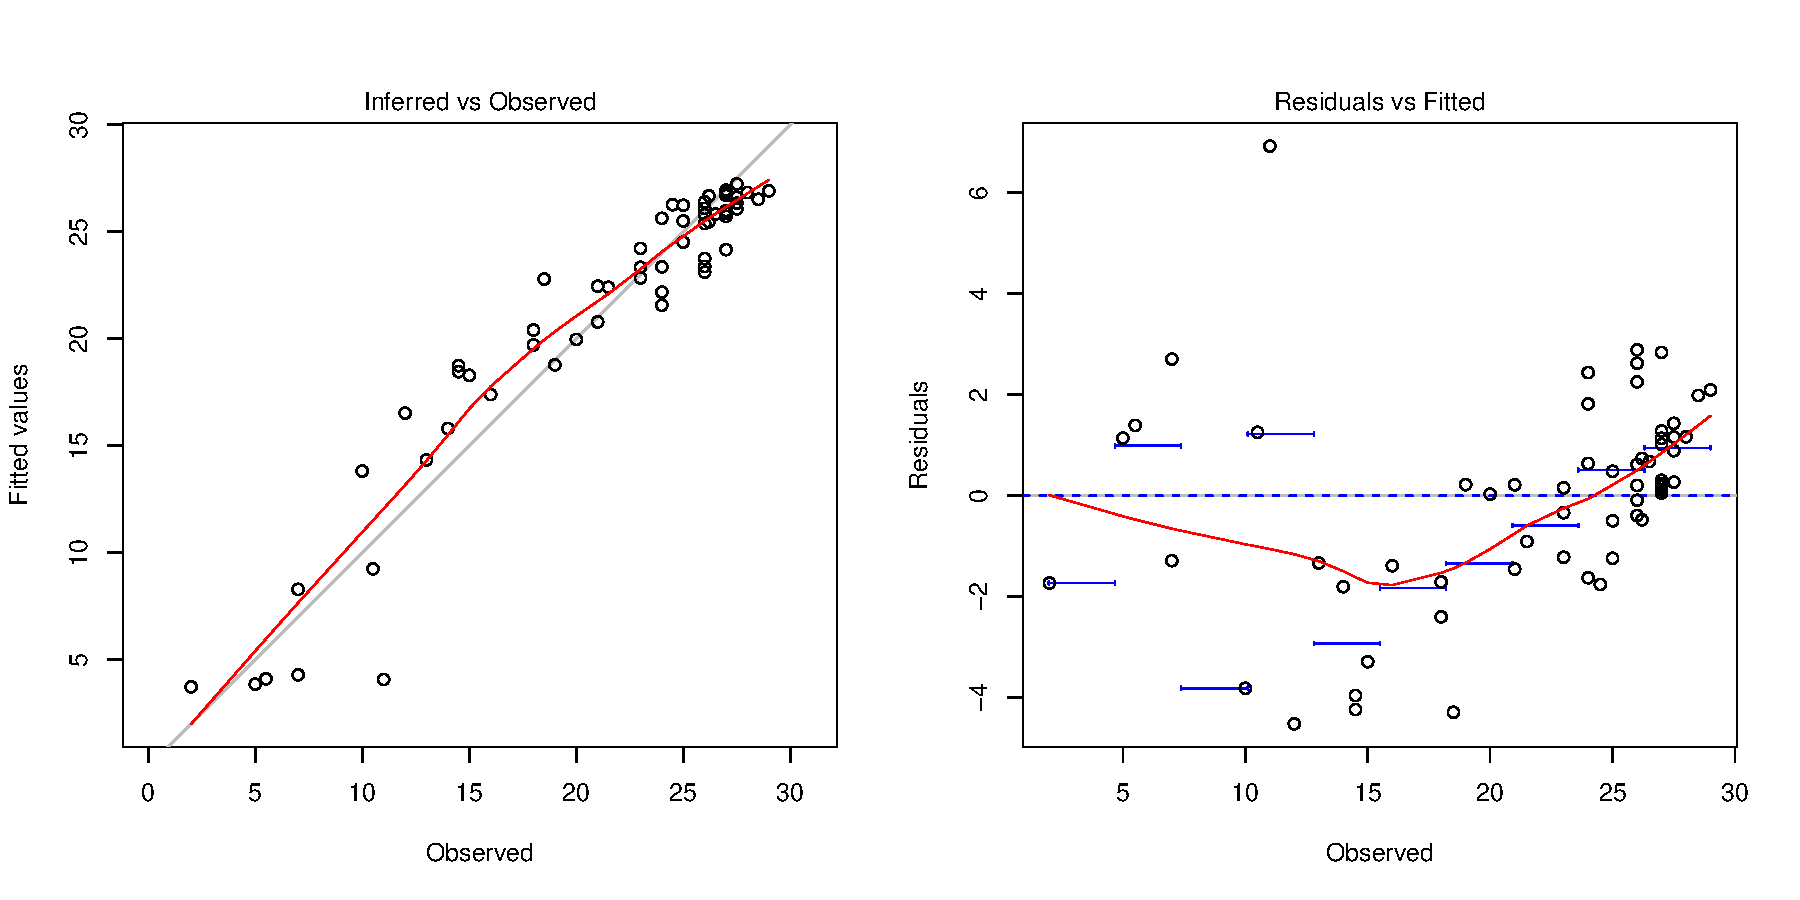
\includegraphics[width=11cm]{wa_diag_plots}
    \end{center}
\end{frame}

\begin{frame}[fragile,allowframebreaks]
    \frametitle{WA --- predictions}
    \scriptsize
\begin{Schunk}
\begin{Sinput}
r$> pred <- predict(mod, imbrie.fos)
r$> pred
\end{Sinput}
\begin{Soutput}
	Weighted Averaging Predictions

Call:
predict(object = mod, newdata = imbrie.fos) 

Deshrinking     : Inverse 
Crossvalidation : none 
Tolerance DW    : No 

Performance:
   RMSEP        R2  Avg.Bias  Max.Bias  
  2.0188    0.9173    0.0000   -3.8155  

Predictions:
      0      10      20      30      40      50      60      70      80 
26.8321 26.7870 26.5611 26.1722 26.1857 26.1670 25.9064 26.0574 26.2797 
     90     100     110     120     130     140     150     160     170 
25.6723 26.1054 25.6092 25.8379 25.7696 25.7891 26.0105 25.8400 26.1986 
    180     190     200     210     220     230     240     250     260 
26.0054 26.4729 26.4282 26.5318 26.7689 26.7812 26.8077 26.0786 26.4078 
    270     280     290     300     310     320     330     340     350 
26.3981 26.1494 26.4148 26.2799 25.8553 26.0269 25.3974 26.0271 26.2423 
    360     370     380     390     400     410     420     430     440 
26.3020 26.7047 26.7140 26.2727 25.4927 26.7538 26.6039 26.6019 26.1936 
    450     460     470     480     490     500     510     520     530 
26.7939 26.7742 26.2152 25.4620 26.7682 26.8107 26.2679 25.7851 25.8562 
    540     550     560     570     580     590     600     610     620 
25.5992 25.0000 25.3488 25.3794 25.3995 26.5347 26.1509 26.1765 26.1447 
    630     640     650     660     670     680     690     700     710 
25.8472 26.3835 26.3507 26.0932 24.5383 25.3052 26.6331 26.3173 26.4848 
    720     730     740     750     760     770     780     790     800 
26.0882 26.1193 26.1579 26.0043 26.3400 26.6920 26.9768 26.9926 26.8074 
    810     820     830     840     850     860     870     880     890 
26.4448 25.4736 25.8549 26.0450 26.2881 25.6021 26.1688 25.8223 24.1910 
    900     910     920     930     940     950     960     970     980 
24.4447 24.9817 25.4642 26.2359 26.4497 26.2772 26.1387 26.1874 25.8485 
    990    1000    1010    1020    1030    1040    1050    1060    1070 
25.7372 25.8538 24.8725 24.1065 24.4843 24.1864 25.6200 25.1869 24.8619 
   1080    1090 
26.0186 25.6395 
\end{Soutput}
\end{Schunk}
    \normalsize
\end{frame}

\begin{frame}[fragile]
    \frametitle{Plotting reconstructions}
    \scriptsize
\begin{Schunk}
\begin{Sinput}
r$> reconPlot(pred, use.labels = TRUE, ylab = "SumSST", xlab = "Depth")
\end{Sinput}
\end{Schunk}
    \normalsize
    \begin{center}
    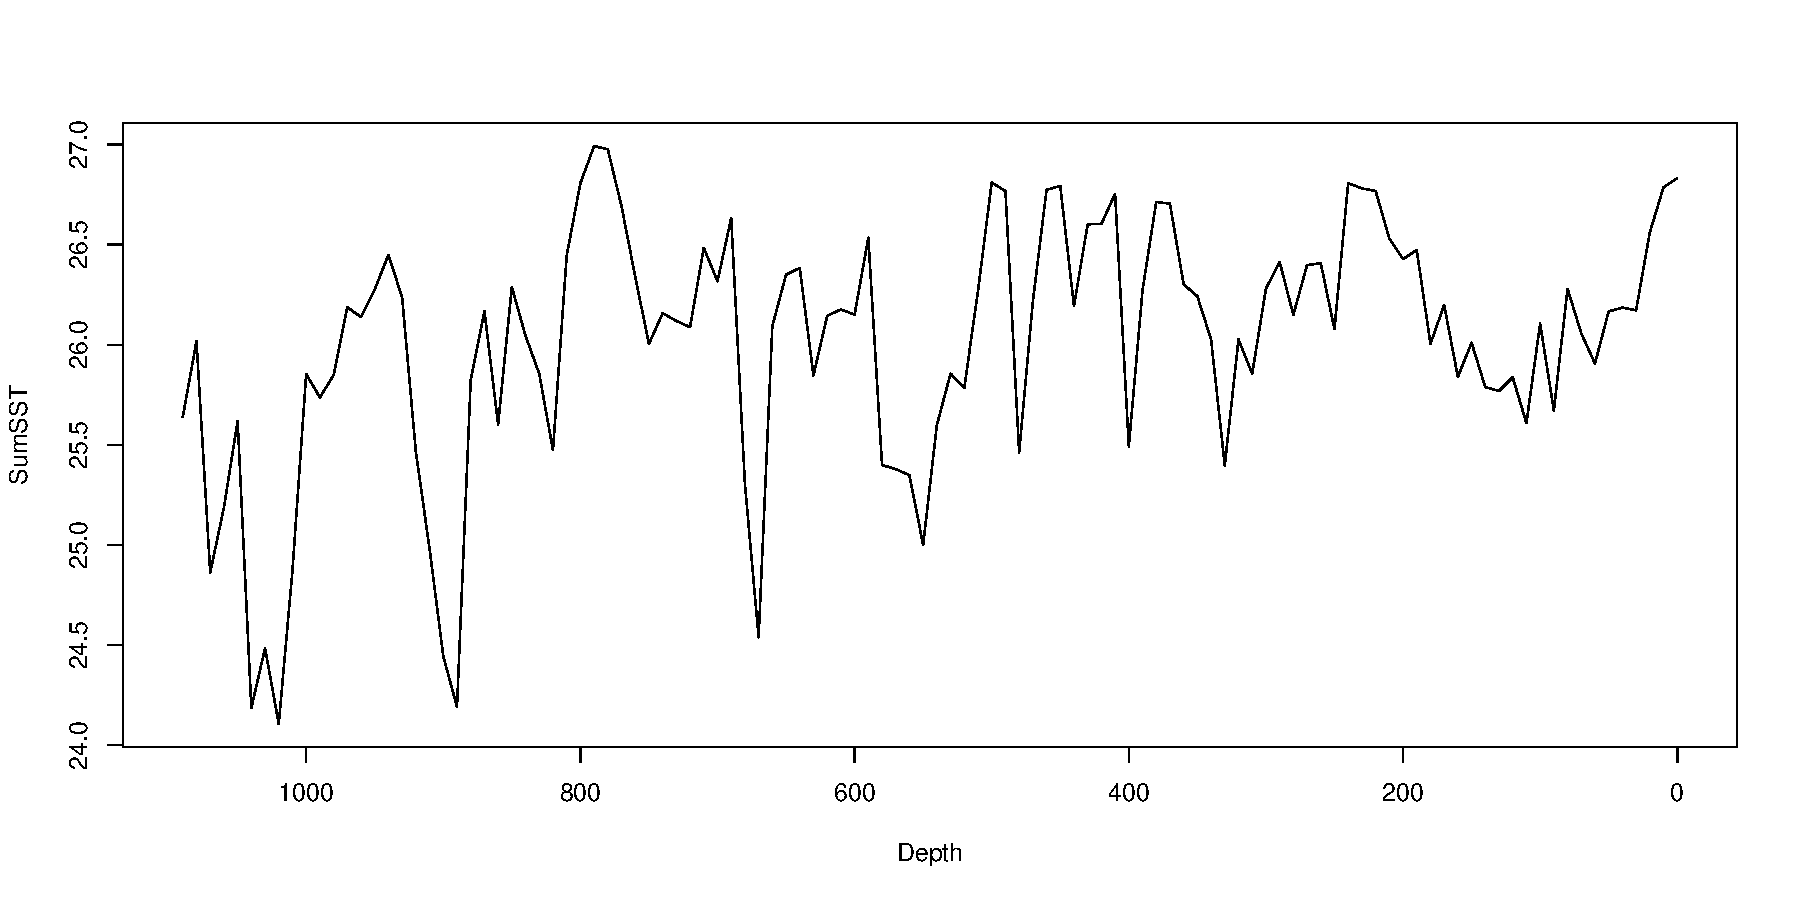
\includegraphics[width=11cm]{reconPlot}
    \end{center}
\end{frame}

\section{Modern Analogue Technique}

\begin{frame}
    \frametitle{Modern Analogue Technique}
    \begin{itemize}
        \item WA take a species approach to reconstruction --- each species in the fossil sample that is also in the training set contributes to the reconstructed values
        \item MAT takes a more holistic approach --- we predict on basis of similar assemblages
        \item In MAT, only the most similar assemblages contribute to the fitted values
        \item MAT is steeped in the tradition of \alert{uniformitarianism} --- \alert{the present is the key to the past}
        \item We take as our prediction of the environment of the past, the (possibly weighted) average of the environment of the $k$ sites with the most similar assemblages
        \item Several things to define; $k$, (dis)similarity
        \item MAT is $k$ nearest neighbours ($k$-NN) regression/calibration
    \end{itemize}
\end{frame}


\begin{frame}
   \frametitle{Measuring association --- binary data}
   \begin{columns}
      \column{5cm}
      \begin{table}
         \begin{tabular}{c|ccc|}
          & \multicolumn{3}{c}{Object $j$}  \\
         \hline
          & & $+$ & $-$ \\
         Object $i$ & $+$ & a & b \\
          & $-$ & c & d \\
         \hline
         \end{tabular}
      \end{table}
      \begin{block}{Jaccard similarity}
         $$s_{ij} = \frac{a}{a + b + c}$$
      \end{block}
      \begin{block}{Jaccard dissimilarity}
         $$d_{ij} = \frac{b + c}{a + b + c}$$
      \end{block}

      \column{5cm}
      \begin{itemize}
         \item Dissimilarity based on the number of species present only in $i$ ($b$), or $j$ ($c$), or in present in both ($a$), or absent in both ($d$).
      \end{itemize}
      \begin{block}{Simple matching coefficient}
         $$s_{ij} = \frac{a + d}{a + b + c + d}$$
      \end{block}
      \begin{block}{Simple matching coefficient}
         $$d_{ij} = \frac{b + c}{a + b + c + d}$$
      \end{block}
   \end{columns}

\end{frame}

\begin{frame}
   \frametitle{Measuring association --- quantitative data}
   \begin{columns}
      \column{6cm}
      \includegraphics[width=6cm]{euclidean_diag}

      \column{4cm}
      \begin{block}{Euclidean distance}
         $d_{ij} = \sqrt{\sum\limits^m_{k=1}(x_{ik} - x_{jk})^2}$
      \end{block}
      \begin{block}{Manhattan distance}
         $d_{ij} = \sum\limits^m_{k=1}|x_{ik} - x_{jk}|$
      \end{block}
      \begin{block}{Bray-Curtis}
         $d_{ij} = \frac{\sum\limits^m_{k=1}|x_{ik} - x_{jk}|}{\sum\limits^m_{k=1}(x_{ik} + x_{jk})}$
      \end{block}
   \end{columns}

\end{frame}

\begin{frame}
   \frametitle{Measuring association --- quantitative data}
   \begin{columns}
      \column{7cm}
      \begin{itemize}
         \item Euclidean distance dominated by large values.
         \item Manhattan distance less affected by large values.
         \item Bray-Curtis sensitive to extreme values.
         \item Similarity ratio (Steinhaus-Marczewski $\equiv$ Jaccard) less dominated by extremes.
         \item Chord distance, used for proportional data; \alert{signal-to-noise} measure.
      \end{itemize}

      \column{5cm}
      \begin{block}{Similarity ratio}
         $d_{ij} = \frac{\sum\limits^m_{k=1}x_{ik}x_{jk}}{\left(\sum\limits^m_{k=1}x_{ik}^2 + \sum\limits^m_{k=1}x_{jk}^2 - \sum\limits^m_{k=1}x_{ik}x_{jk}\right)^2}$
      \end{block}
      \begin{block}{Chord distance}
         $d_{ij} = \sqrt{\sum\limits^m_{k=1}(\sqrt{p_{ik}} - \sqrt{p_{jk}})^2}$
      \end{block}
   \end{columns}
\end{frame}

\begin{frame}
   \frametitle{Measuring association --- mixed data}
   \begin{block}{Gower's coefficient}
   $$s_{ij} = \frac{\sum\limits^m_{i=1} w_{ijk}s_{ijk}}{\sum\limits^m_{i=1} w_{ijk}}$$
   \end{block}
   \begin{itemize}
      \item $s_{ijk}$ is similarity between sites $i$ and $j$ for the $k$th variable.
      \item Weights $w_{ijk}$ are typically 0 or 1 depending on whether the comparison is valid for variable $k$. Can also use variable weighting with $w_{ijk}$ between 0 and 1.
      \item $w_{ijk}$ is zero if the $k$th variable is missing for one or both of $i$ or $j$.
      \item For binary variables $s_{ijk}$ is the Jaccard coefficient.
      \item For categorical data $s_{ijk}$ is 1 of $i$ and $k$ have same category, 0 otherwise.
      \item For quantitative data $s_{ijk} = (1 - |x_{ik} - x_{jk}|) / R_k$
   \end{itemize}
\end{frame}

\begin{frame}
    \frametitle{MAT}
    \begin{itemize}
        \item Once you have chosen a suitable dissimilarity coefficient, MAT begins
        \item We calculate the dissimilarity between each training set sample and every other
        \item For each site in turn, we order the training set samples in terms of increasing dissimilarity to the target training set sample
        \item Calculate the (weighted) average of the environment for the closest site, then the two closest sites, then the three closest sites, ... and so on
        \item The weights, if used, are the inverse of the dissimilarity $w_{jk} = 1 / d_{jk}$
        \item For each model of size $k$ we calculate some performance statistics
        \item Choose as our model, the $k$ that achieves the lowest RMSEP across the whole training set
        \item Very simple!
    \end{itemize}
\end{frame}

\begin{frame}[fragile, allowframebreaks]
    \frametitle{MAT in analogue}
    \scriptsize
\begin{Schunk}
\begin{Sinput}
r$> data(swapdiat, swappH, rlgh)
r$> dat <- join(swapdiat, rlgh, verbose = TRUE)
\end{Sinput}
\begin{Soutput}
Summary:

            Rows Cols
Data set 1:  167  277
Data set 2:  101  139
Merged:      268  277
\end{Soutput}
\begin{Sinput}
r$> swapdiat <- with(dat, swapdiat / 100)
r$> rlgh <- with(dat, rlgh / 100)
r$> swap.mat <- mat(swappH ~ ., data = swapdiat, method = "SQchord")
r$> swap.mat
\end{Sinput}
\begin{Soutput}
	Modern Analogue Technique

Call:
mat(formula = swappH ~ ., data = swapdiat, method = "SQchord") 

Percentiles of the dissimilarities for the training set:

   1%    2%    5%   10%   20% 
0.416 0.476 0.574 0.668 0.815 

Inferences based on the mean of k-closest analogues:

  k   RMSEP      R2 Avg Bias Max Bias
  1  0.4227  0.7139  -0.0254  -0.3973
  2  0.3741  0.7702  -0.0493  -0.4689
  3  0.3387  0.8088  -0.0379  -0.4034
  4  0.3282  0.8200  -0.0335  -0.4438
  5  0.3136  0.8356  -0.0287  -0.4124
  6  0.3072  0.8444  -0.0386  -0.4152
  7  0.3167  0.8364  -0.0481  -0.4179
  8  0.3065  0.8474  -0.0433  -0.4130
  9  0.3049  0.8495  -0.0436  -0.4111
 10  0.3015  0.8548  -0.0473  -0.4083

Inferences based on the weighted mean of k-closest analogues:

  k   RMSEP      R2 Avg Bias Max Bias
  1  0.4227  0.7139  -0.0254  -0.3973
  2  0.3711  0.7734  -0.0476  -0.4614
  3  0.3375  0.8102  -0.0385  -0.4088
  4  0.3272  0.8213  -0.0346  -0.4433
  5  0.3144  0.8348  -0.0298  -0.4205
  6  0.3077  0.8435  -0.0371  -0.4253
  7  0.3148  0.8377  -0.0451  -0.4250
  8  0.3049  0.8483  -0.0407  -0.4206
  9  0.3035  0.8500  -0.0408  -0.4205
 10  0.3005  0.8546  -0.0442  -0.4180
\end{Soutput}
\end{Schunk}
    \normalsize
\end{frame}

\begin{frame}
    \frametitle{MAT in analogue}
    \begin{itemize}
        \item The RMSEP here is a leave-one-out RMSEP
        \item Each prediction for training set sample $i$ is produced on the basis of using all sites other than $i$
        \item \textbf{analogue} is unique (as far as I know) as it evaluates all $k$ models at once
        \item This means it is slow at times...
        \item ...But you only need to do the fitting once to determine the model with lowest RMSEP
    \end{itemize}
\end{frame}

\begin{frame}[fragile]
    \frametitle{MAT diagnostic plots}
    \begin{columns}
    \column{5cm}
    \scriptsize
\begin{Schunk}
\begin{Sinput}
r$> opar <- par(mfrow = c(2,2))
r$> plot(swap.mat)
r$> par(opar)
\end{Sinput}
\end{Schunk}
    \normalsize
    
    \column{7cm}
    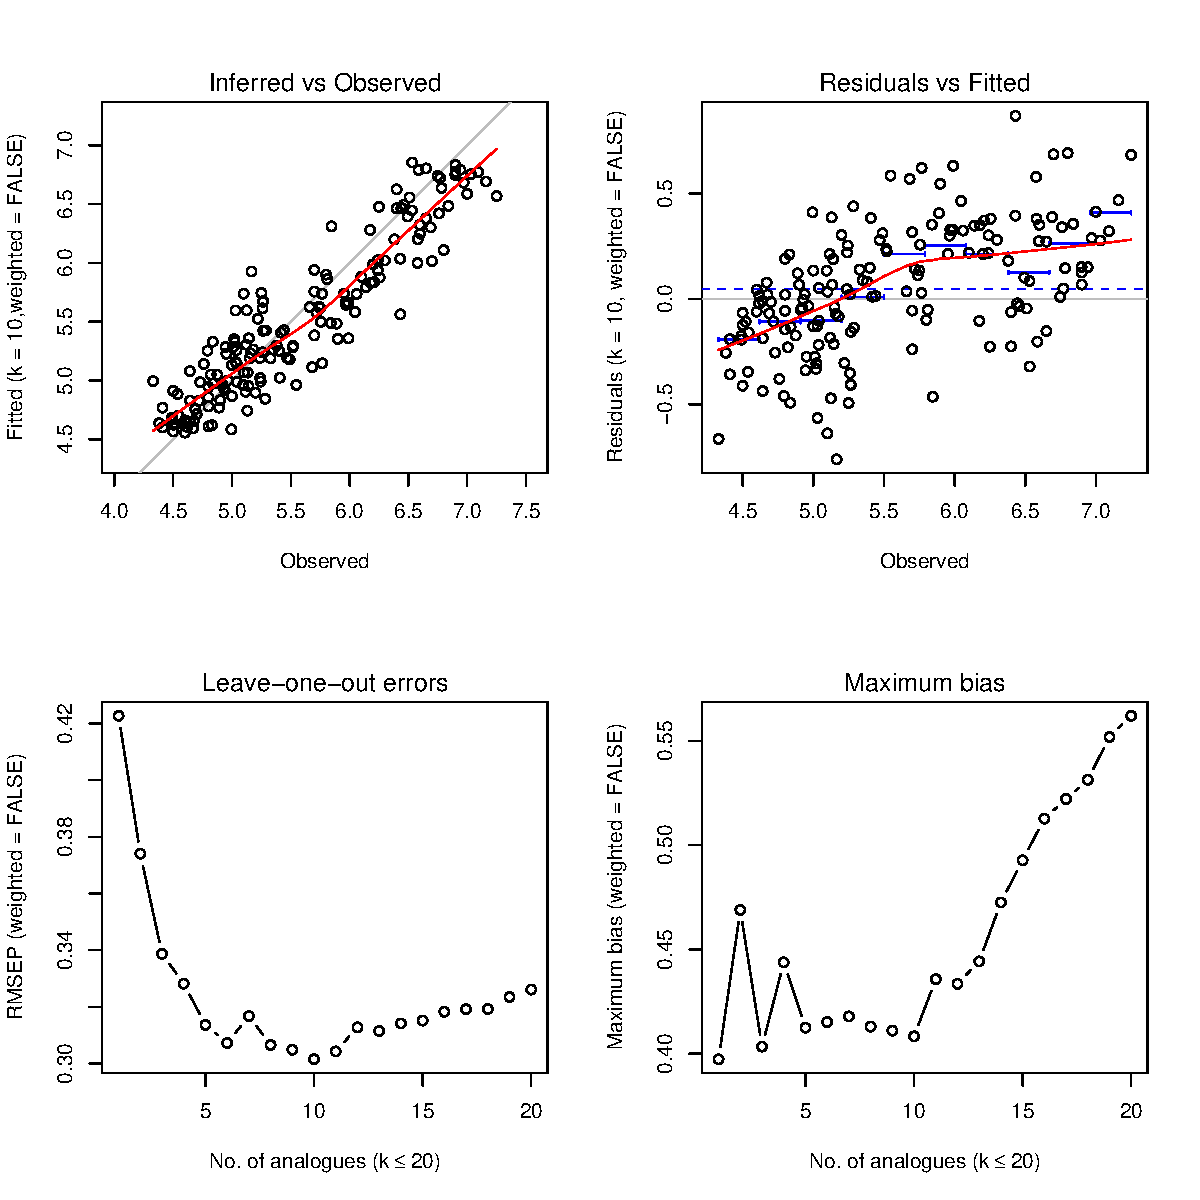
\includegraphics[width=7cm]{mat_diag_plots}
    \end{columns}
\end{frame}

\begin{frame}[fragile, allowframebreaks]
    \frametitle{MAT predictions}
    \begin{itemize}
        \item To make a prediction for a fossil sample using MAT:
        \item Calculate dissimilarity between each fossil sample and each training set sample
        \item Take the $k$ closest training set samples for each fossil sample
        \item The prediction for a fossil sample is the (weighted) average of these $k$ closest training set samples
    \end{itemize}

    \scriptsize
\begin{Schunk}
\begin{Sinput}
r$> rlgh.mat <- predict(swap.mat, rlgh, k = 10)
r$> rlgh.mat
\end{Sinput}
\begin{Soutput}
	Modern Analogue Technique predictions

Dissimilarity: SQchord 
k-closest analogues: 10,	Chosen automatically? FALSE
Weighted mean: FALSE 
Bootstrap estimates: FALSE 

Model error estimates:
    RMSEP r.squared  avg.bias  max.bias 
   0.3015    0.8548   -0.0473   -0.4083 

Predicted values:
000.3 000.8 001.3 001.8 002.3 002.8 003.3 003.8 004.3 004.8 005.3 006.3 
 4.82  4.79  4.83  4.78  4.79  4.82  4.79  4.84  4.79  4.87  4.84  4.90 
007.3 008.3 009.3 010.3 011.8 013.3 014.3 015.3 016.3 017.3 018.3 019.3 
 4.88  5.01  5.10  5.12  5.13  5.26  5.50  5.43  5.43  5.36  5.32  5.36 
020.3 022.3 024.3 025.3 026.3 027.3 028.3 030.5 032.5 036.5 040.5 044.5 
 5.37  5.40  5.50  5.36  5.37  5.48  5.36  5.36  5.47  5.57  5.36  5.55 
048.5 052.5 056.5 060.5 064.5 068.5 072.5 076.5 080.5 084.5 088.5 092.5 
 5.63  5.75  5.72  5.57  5.42  5.44  5.62  5.75  5.51  5.51  5.35  5.51 
096.5 100.5 104.5 108.5 112.5 118.5 120.5 124.5 128.5 130.5 132.5 134.5 
 5.47  5.43  5.46  5.41  5.48  5.31  5.51  5.60  5.66  5.40  5.25  5.41 
136.5 138.5 140.5 142.5 144.5 146.5 148.5 150.5 152.5 154.5 156.5 158.5 
 5.41  5.45  5.49  5.43  5.01  5.23  5.27  5.27  5.27  5.27  5.27  5.31 
160.5 162.5 164.5 166.5 168.5 170.5 172.5 174.5 176.5 178.5 180.5 182.5 
 5.27  5.27  5.25  5.28  5.28  5.23  5.24  5.27  5.27  5.27  5.20  5.23 
184.5 188.5 192.5 196.5 200.5 204.5 208.5 212.5 216.5 220.5 224.5 228.5 
 5.20  5.23  5.30  5.23  5.20  5.21  5.21  5.22  5.20  5.19  5.57  5.61 
244.5 248.5 252.5 254.5 256.5 
 5.59  5.59  5.61  5.69  5.62 
\end{Soutput}
\end{Schunk}
    \normalsize
\end{frame}

\begin{frame}[fragile]
    \frametitle{MAT reconstructions}
    \scriptsize
\begin{Schunk}
\begin{Sinput}
r$> reconPlot(rlgh.mat, use.labels = TRUE, ylab = "pH", xlab = "Depth (cm.)")
\end{Sinput}
\end{Schunk}
    \normalsize
    \begin{center}
        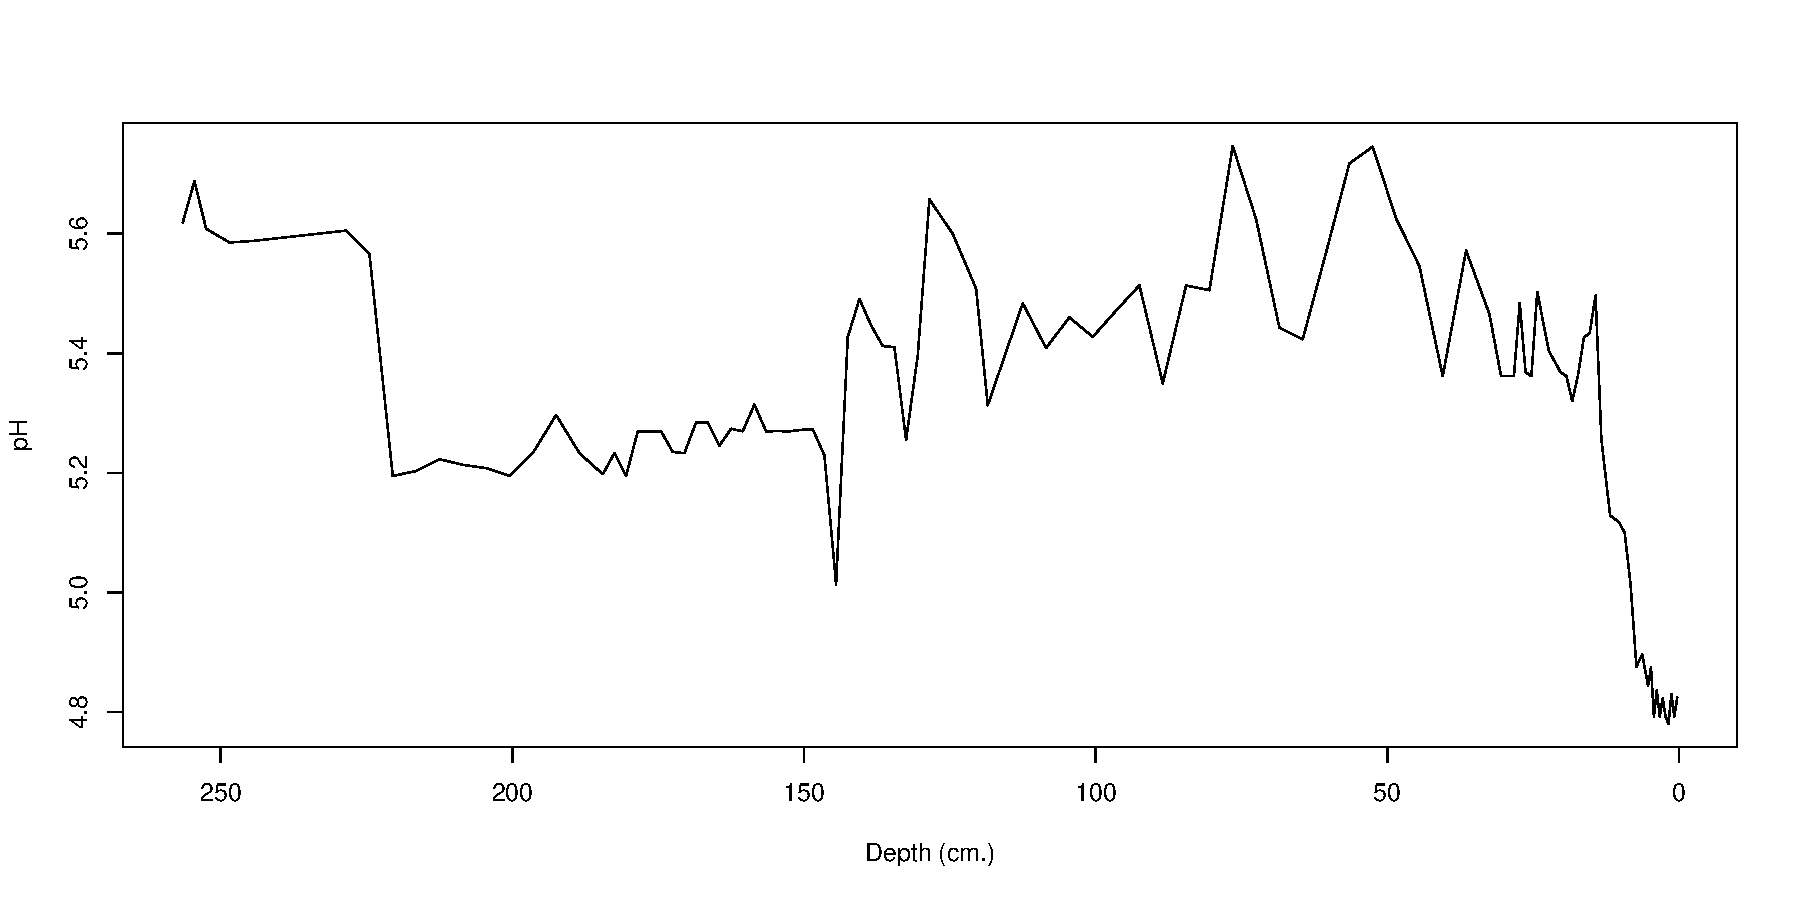
\includegraphics[width=11cm]{mat_reconPlot}
    \end{center}
\end{frame}

\section{Model performance and diagnostics}

\begin{frame}
    \frametitle{Bias}
    \begin{columns}
        \column{7cm}
        \begin{itemize}
            \item Bias is the tendency for the model to over or under predict
            \item Average bias is the mean of the residuals
            \item Maximum bias is found by breaking the range of the measured environment into $n$ contiguous chunks ($n = 10$ usually)
            \item Within each chunk calculate the mean of the residuals for that chunk
            \item Take the maximum value of these as the maximum bias statistic
        \end{itemize}

        \column{5cm}
        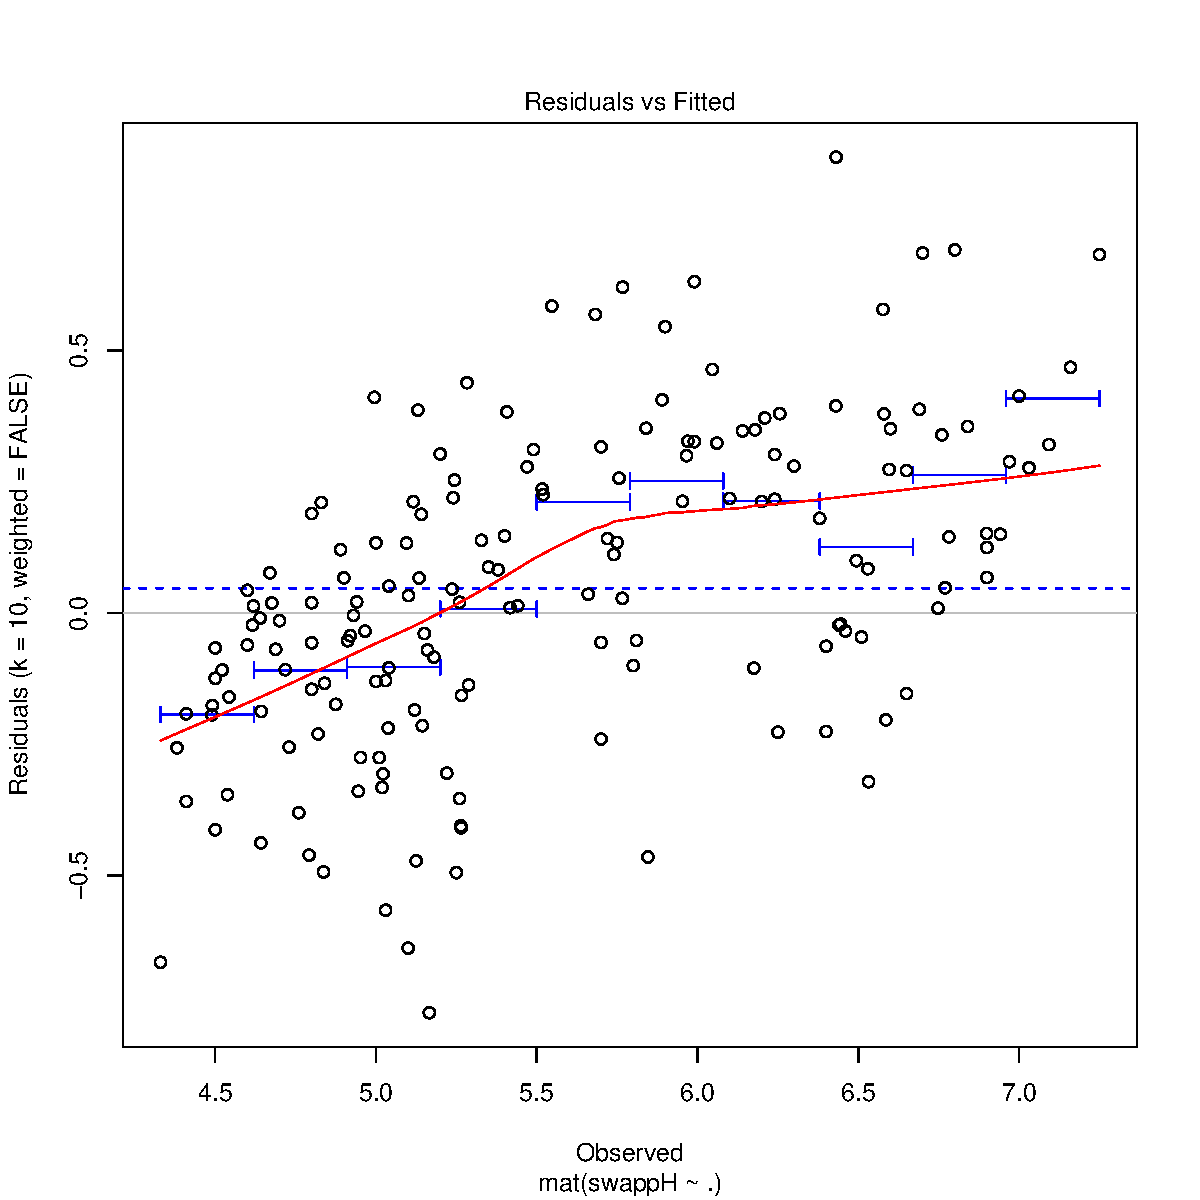
\includegraphics[width=5cm]{mat_bias_plot}
    \end{columns}
\end{frame}

\begin{frame}
    \frametitle{Cross-validation}
    \begin{itemize}
        \item Without cross-validation, prediction errors, measured by RMSEP, will be biased, often badly so
        \item This is because we use the same data to both fit \alert{and} test the model
        \item Ideally we'd have such a large training set that we can split this into a slightly smaller training set and a small test set
        \item Palaeoecological data is expensive to obtain --- in money and person-hours!
        \item Also these ecosystems are complex, species rich, noisy etc., so we want to use all our data to produce a model
        \item One solution to this problem is to use cross-validation
        \item General idea is we perturb our training set in some way, build a new model on the perturbed training set and assess how well it performs
        \item If we repeat the perturbation several time we get an idea of the error in the model
        \item Several techniques; $n$-fold, leave-one-out, bootstrapping (aka \alert{bagging})
    \end{itemize}
\end{frame}

\begin{frame}
    \frametitle{Cross-validation in \textbf{analogue}}
    \begin{itemize}
        \item In \textbf{analogue}, several methods are available
        \item For MAT models, LOO is built into the procedure so only bootstrapping is available
        \item For WA models, both LOO and bootstrapping currently available
        \item $n$-fold CV will be available in a future version
    \end{itemize}
\end{frame}

\begin{frame}[fragile]
    \frametitle{LOO Cross-validation in \textbf{analogue}}
    \begin{itemize}
        \item LOO CV is very simple
        \item In turn, leave out each sample from the training set
        \item Build a model on the remaining samples
        \item Predict for the left out sample
        \item Calculate the RMSEP of these predictions
    \end{itemize}
    \scriptsize
\begin{Schunk}
\begin{Sinput}
r$> loo.pred <- predict(mod, imbrie.fos, CV = "LOO", verbose = TRUE)
\end{Sinput}
\begin{Soutput}
Leave one out sample 10 
Leave one out sample 20 
Leave one out sample 30 
Leave one out sample 40 
Leave one out sample 50 
Leave one out sample 60 
\end{Soutput}
\begin{Sinput}
r$> performance(mod)
\end{Sinput}
\begin{Soutput}
    RMSE       R2 Avg.Bias Max.Bias 
   2.019    0.917    0.000   -3.815 
\end{Soutput}
\begin{Sinput}
r$> performance(loo.pred)
\end{Sinput}
\begin{Soutput}
   RMSEP       R2 Avg.Bias Max.Bias 
   2.218    0.900   -0.014   -4.599 
\end{Soutput}
\end{Schunk}
    \normalsize
\end{frame}

\begin{frame}
    \frametitle{Bootstrap Cross-validation in \textbf{analogue}}
    \begin{itemize}
        \item Bootstrapping used in machine learning to improve predictions
        \item Use bootstrapping to get more realistic RMSEP and bias statistics
        \item We draw a bootstrap sample (sampling with replacement) of the same size as our training set
        \item Build a model on the bootstrap samples
        \item Predict for the out-of-bag (OOB) samples
        \item Bootstrap prediction for each model sample is the mean of the OOB prediction for each sample
        \item Calculate the residuals and then the RMSEP
        $$\mathrm{RMSEP_{boot}} = \sqrt{s_1^2 + s_2^2}$$
        \item $s_1^2$ is the standard deviation of the OOB residuals
        \item $s_2^2$ is the mean of the OOB residuals
        \item We can also calculate the more usual RMSEP $\sqrt{\sum_{i=1}^n (y_i - \hat{y}_i)^2 / n}$
    \end{itemize}
    
\end{frame}

\begin{frame}[fragile]
    \frametitle{Bootstrap Cross-validation in \textbf{analogue}}
    \scriptsize
\begin{Schunk}
\begin{Sinput}
r$> set.seed(1234)
r$> swap.boot <- bootstrap(swap.mat, n.boot = 200)
r$> swap.boot
\end{Sinput}
\begin{Soutput}
	Bootstrap results for palaeoecological models

Model type: MAT 
Weighted mean: FALSE 
Number of bootstrap cycles: 200 

Leave-one-out and bootstrap-derived error estimates:

           k RMSEP   S1    S2 r.squared avg.bias max.bias
LOO       10 0.301    -     -     0.855  -0.0473   -0.408
Bootstrap 11 0.327 0.12 0.305     0.924  -0.0501   -0.435
\end{Soutput}
\begin{Sinput}
r$> RMSEP(swap.boot, type = "standard")
\end{Sinput}
\begin{Soutput}
[1] 0.3045873
\end{Soutput}
\end{Schunk}
    \normalsize
\end{frame}

\begin{frame}[fragile]
    \frametitle{Minimum dissimilarity to a training set sample}
    \begin{itemize}
        \item A measure of reliability for the reconstructed values can be determined from the distance between each fossil sample and the training set samples
        \item For a reconstructed value to be viewed as more reliable, it should have at least one close modern analogue in the training set
        \item Close modern analogues are defined as those modern training set samples that are as similar to a fossil sample as a low percentile of the observed distribution dissimilarities in the training set, say the 5$^{th}$ percentile
    \end{itemize}
    \scriptsize
\begin{Schunk}
\begin{Sinput}
r$> rlgh.mdc <- minDC(rlgh.mat)
r$> plot(rlgh.mdc, use.labels = TRUE, xlab = "Depth (cm.)")
r$> quantile(as.dist(swap.mat$Dij), prob = c(0.01,0.025,0.05, 0.1))
\end{Sinput}
\begin{Soutput}
       1%      2.5%        5%       10% 
0.4164113 0.4972167 0.5738378 0.6676391 
\end{Soutput}
\end{Schunk}
    \normalsize
\end{frame}

\begin{frame}[fragile]
    \frametitle{Minimum dissimilarity to a training set sample}
    \scriptsize
\begin{Schunk}
\begin{Sinput}
r$> plot(rlgh.mdc, use.labels = TRUE, xlab = "Depth (cm.)")
r$> quantile(as.dist(swap.mat$Dij), prob = c(0.01,0.025,0.05, 0.1))
\end{Sinput}
\begin{Soutput}
       1%      2.5%        5%       10% 
0.4164113 0.4972167 0.5738378 0.6676391 
\end{Soutput}
\end{Schunk}
    \normalsize
    \begin{center}
        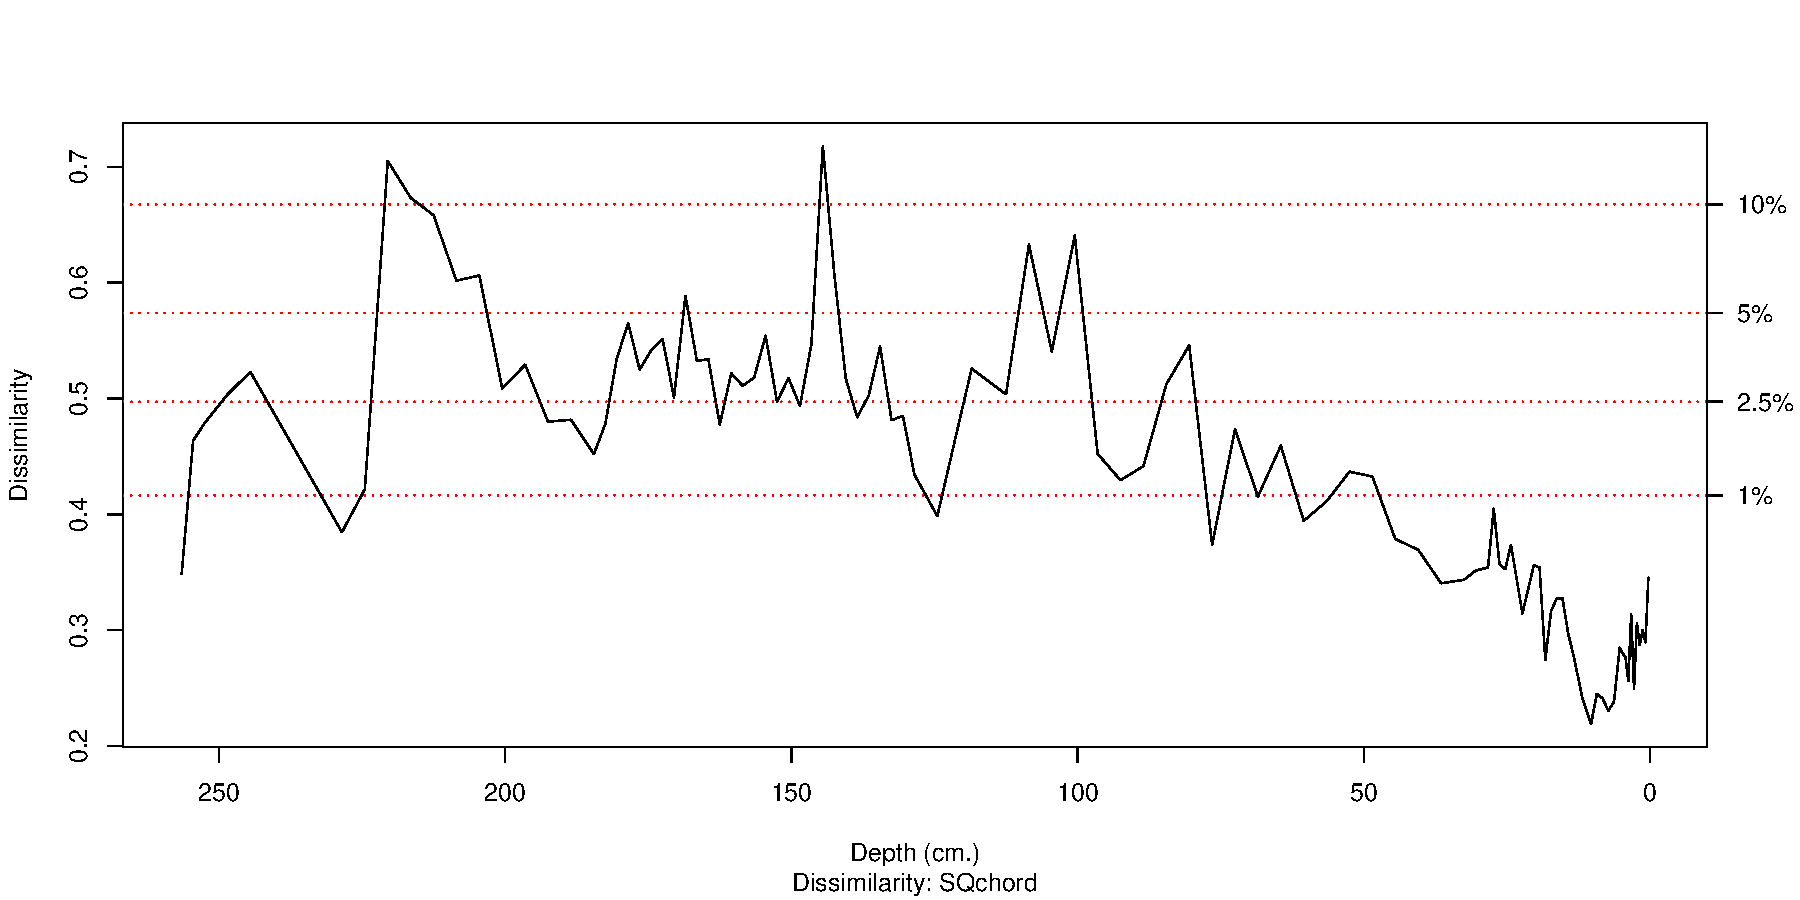
\includegraphics[width=11cm]{minDC_plot}
    \end{center}
\end{frame}

\begin{frame}[fragile]
    \frametitle{Sample-specific error estimates}
    \begin{itemize}
        \item We can use the bootstrap approach to generate sample specific errors for each fossil sample
        $$\mathrm{RMSEP} = \sqrt{s^2_{1_{fossil}} + s^2_{2_{model}}}$$
        \item $s^2_{1_{fossil}}$ is the standard deviation of the bootstrap estimates for the fossil samples
        \item $s^2_{2_{model}}$ is the average bias, the mean of the bootstrap OOB residuals from the model
    \end{itemize}
\end{frame}

\begin{frame}[fragile]
    \frametitle{Sample-specific error estimates}
    \scriptsize
\begin{Schunk}
\begin{Sinput}
r$> swap.boot
\end{Sinput}
\begin{Soutput}
	Bootstrap results for palaeoecological models

Model type: MAT 
Weighted mean: FALSE 
Number of bootstrap cycles: 200 

Leave-one-out and bootstrap-derived error estimates:

           k RMSEP   S1    S2 r.squared avg.bias max.bias
LOO       10 0.301    -     -     0.855  -0.0473   -0.408
Bootstrap 11 0.327 0.12 0.305     0.924  -0.0501   -0.435
\end{Soutput}
\begin{Sinput}
r$> set.seed(1234)
r$> rlgh.boot <- predict(swap.mat, rlgh, bootstrap = TRUE, n.boot = 200)
r$> reconPlot(rlgh.boot, use.labels = TRUE, ylab = "pH", xlab = "Depth (cm.)", display.error = "bars", predictions = "bootstrap")
\end{Sinput}
\end{Schunk}
    \normalsize
\end{frame}

\begin{frame}[fragile]
    \frametitle{Sample-specific error estimates}
    \scriptsize
\begin{Schunk}
\begin{Sinput}
r$> reconPlot(rlgh.boot, use.labels = TRUE, ylab = "pH", xlab = "Depth (cm.)", display.error = "bars", predictions = "bootstrap")
\end{Sinput}
\end{Schunk}
    \normalsize
    \begin{center}
        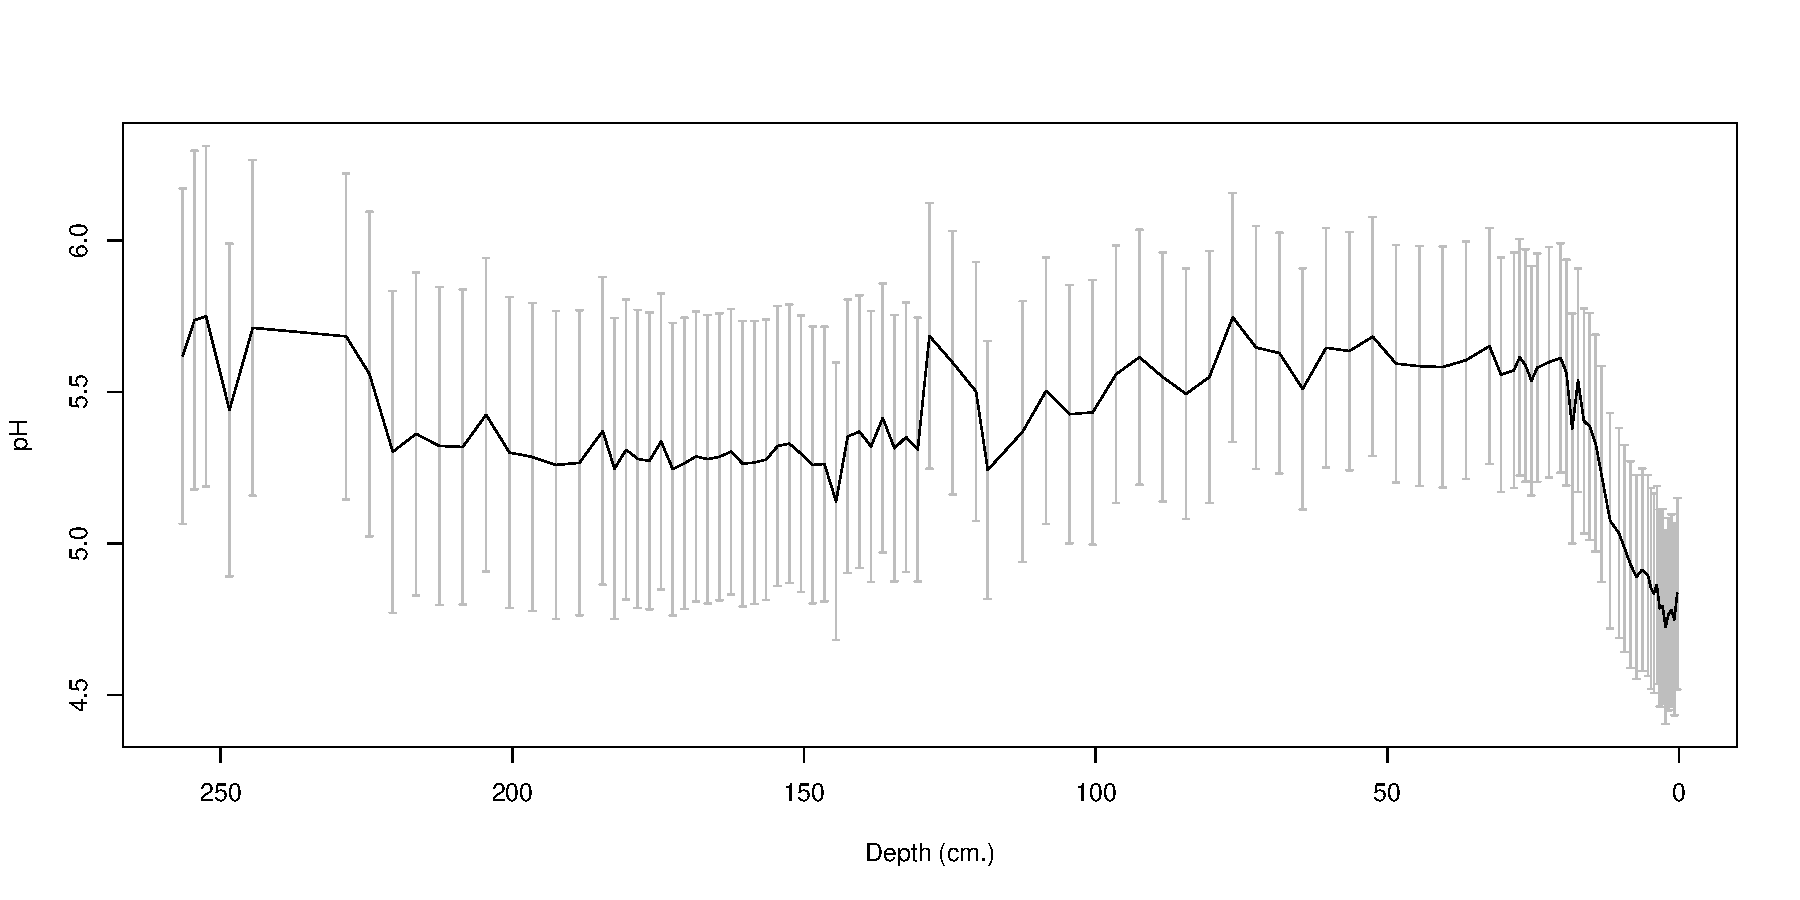
\includegraphics[width=11cm]{sample_specific_error_plot}
    \end{center}
\end{frame}


\section{Odds and ends}

\end{document}
